%\section{Forest Representativeness}
%%%%%%%%%%%%%%%%%%%%%%%%%%%%%%%%%%%%%%%%%%%%%%%%%%%%%%%%%%%%%%%%%%%%%%%%%%%%%%%%
%\begin{frame}
% \frametitle{ForestGEO Network Global Representativeness}
% 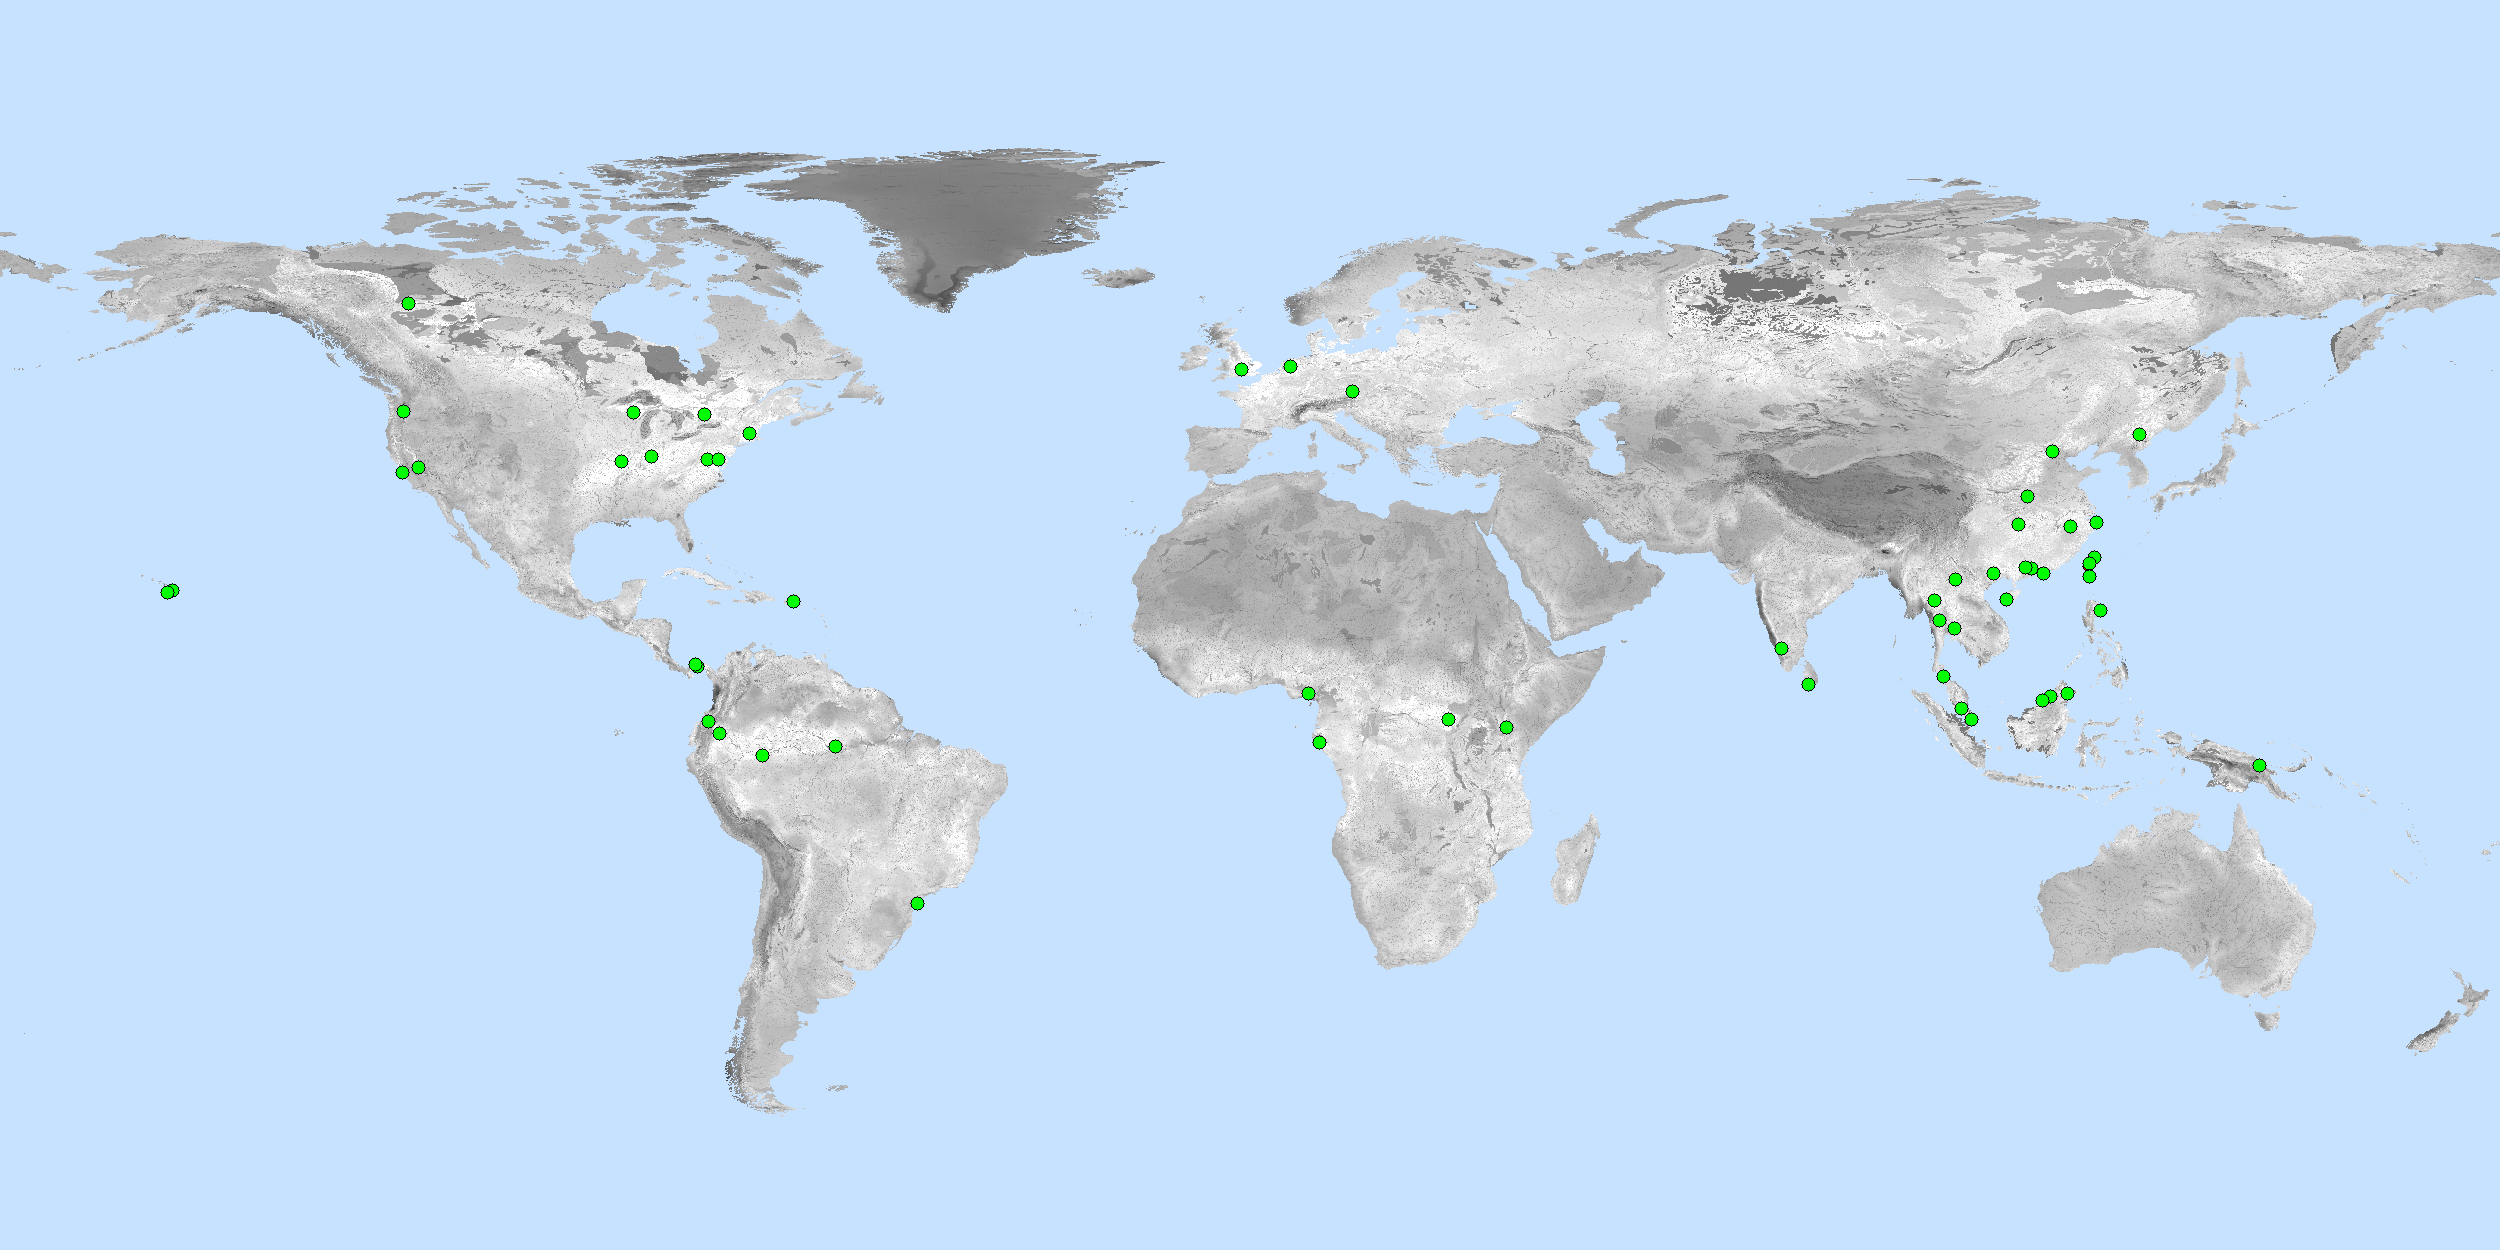
\includegraphics[width=\textwidth]{forest_figures/forestGEOall_years_2013.png} \\
% \vskip-0.25in\vbox{\scriptsize\hfill (Maddalena et al., in prep)}
%
%\smallskip
%Light-colored regions are well represented and dark-colored regions are
%poorly represented by the ForestGEO sampling network.
%
%\smallskip
%Animation of the time evolution of the ForestGEO network: \href{https://climate.ornl.gov/~jkumar/share/forestGEOall_years.gif}{https://climate.ornl.gov/$\sim$jkumar/share/forestGEOall\_years.gif}
%
%\end{frame}
%%%%%%%%%%%%%%%%%%%%%%%%%%%%%%%%%%%%%%%%%%%%%%%%%%%%%%%%%%%%%%%%%%%%%%%%%%%%%%%%

%%%%%%%%%%%%%%%%%%%%%%%%%%%%%%%%%%%%%%%%%%%%%%%%%%%%%%%%%%%%%%%%%%%%%%%%%%%%%%%
\begin{frame}
 \frametitle{Triple-Network Global Representativeness}
 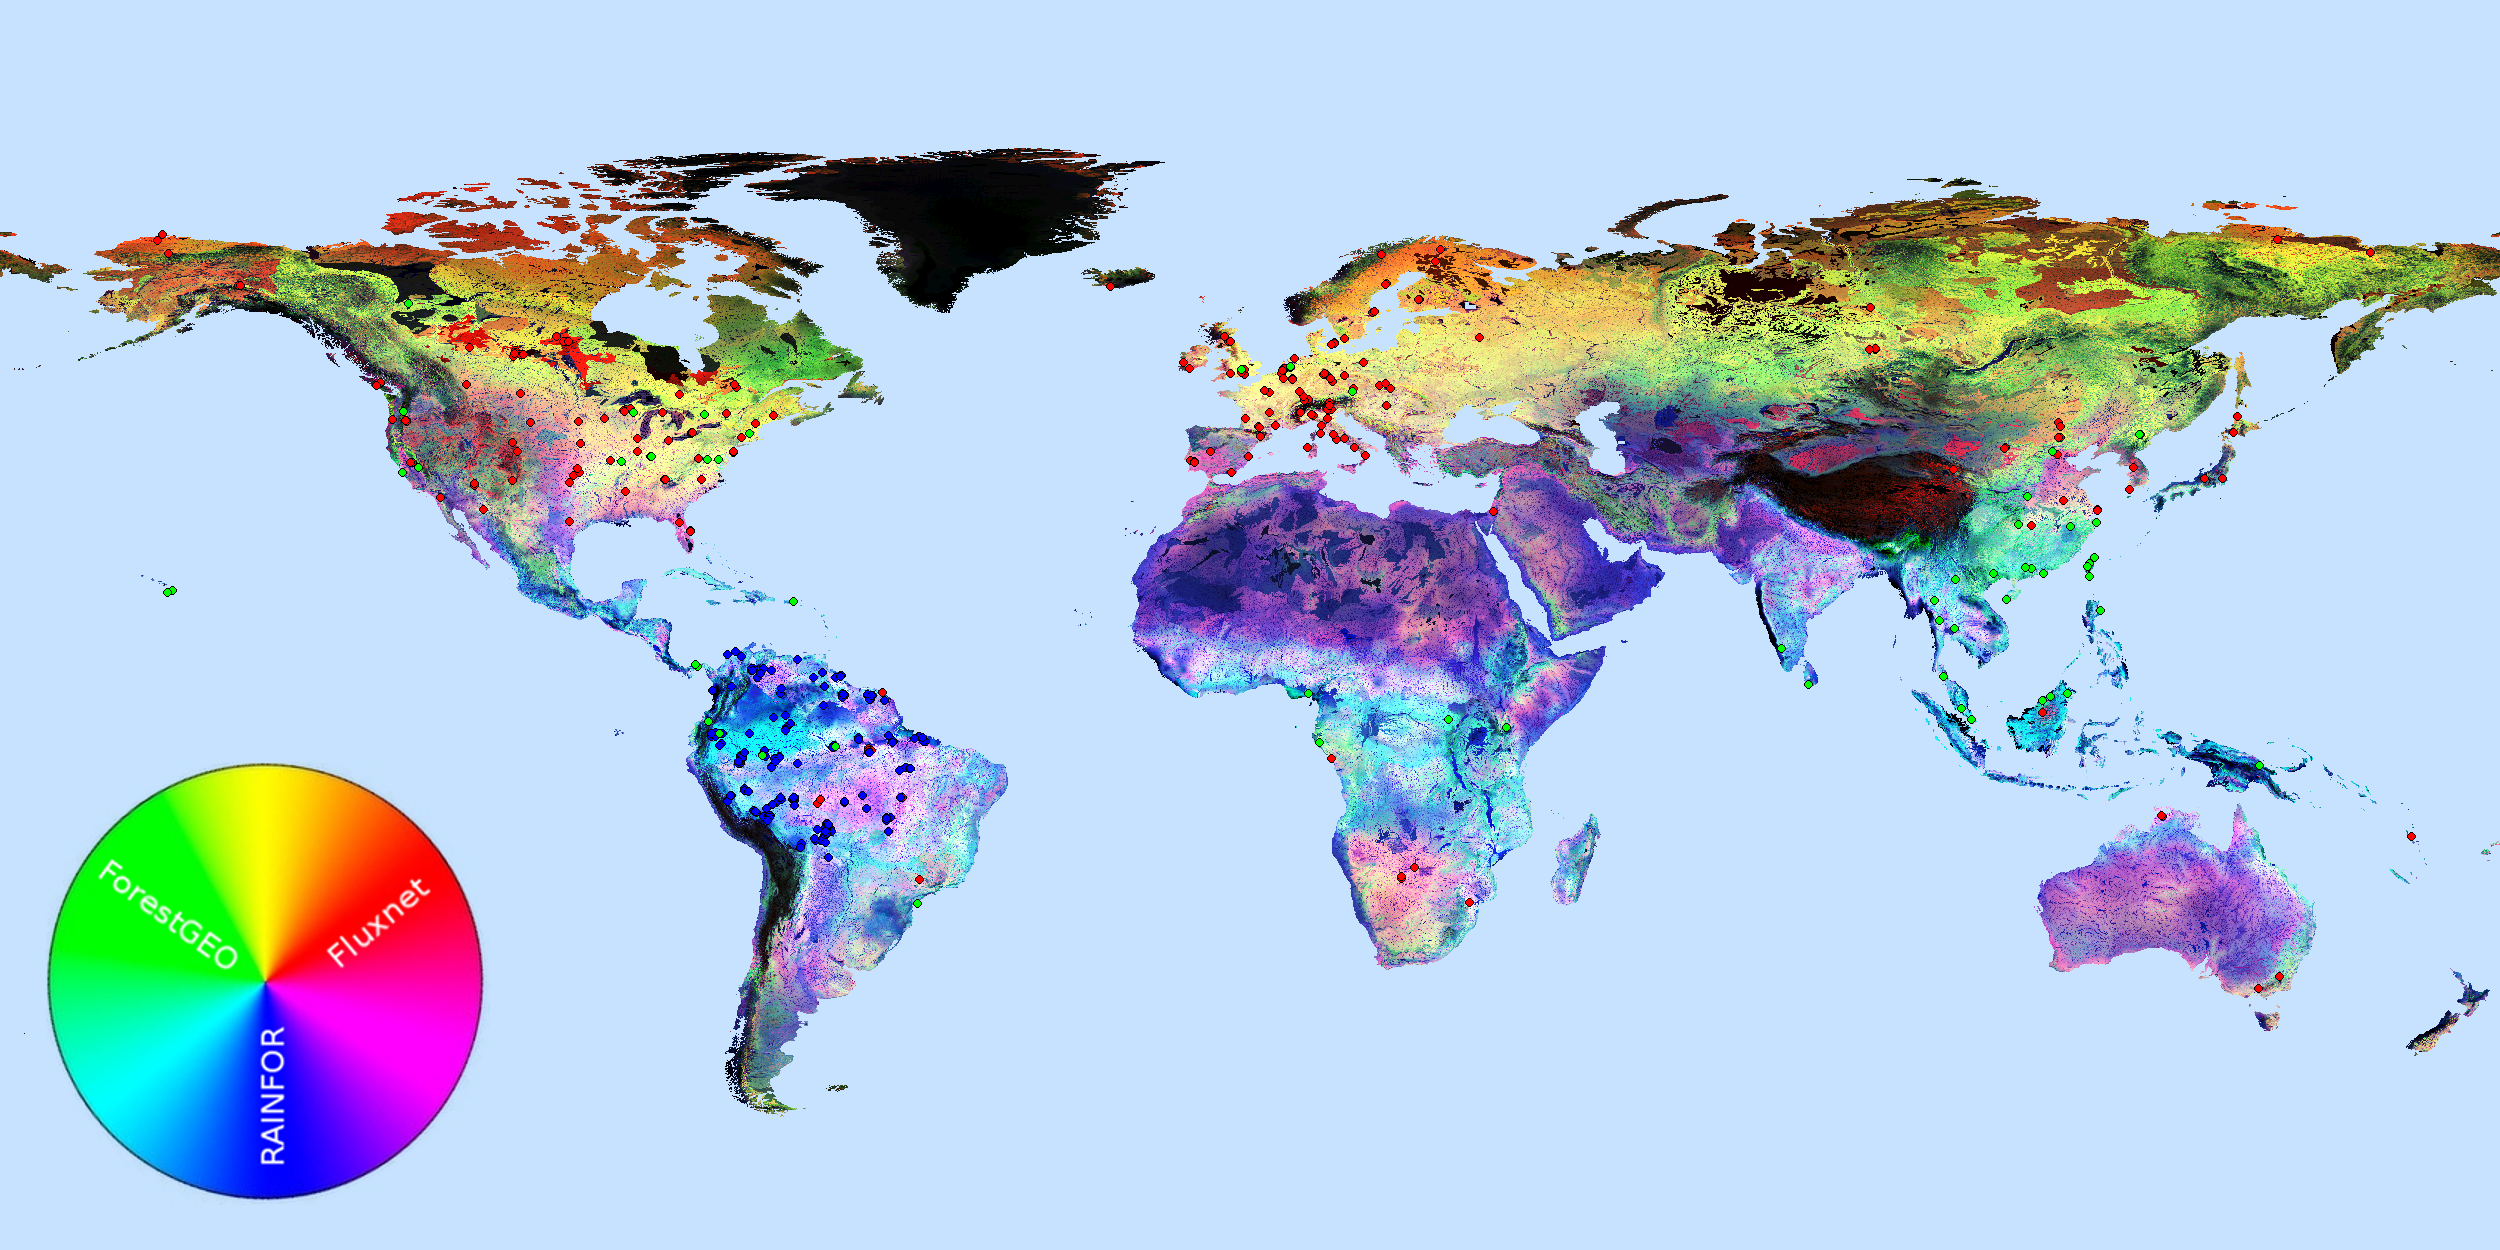
\includegraphics[width=\textwidth]{forest_figures/allNetworks_global_RGB_histEq_wheelLegend.png} \\
 \vskip-0.25in\vbox{\scriptsize\hfill (Maddalena et al., in prep)}

\medskip
Map indicates which sampling network offers the most representative
coverage at any location. Every location is made up of a combination of
three primary colors from Fluxnet (red), ForestGEO (green), and RAINFOR
(blue).

\end{frame}
%%%%%%%%%%%%%%%%%%%%%%%%%%%%%%%%%%%%%%%%%%%%%%%%%%%%%%%%%%%%%%%%%%%%%%%%%%%%%%%

